\chapter{Cellular automata}

%Nejaka citacia od Feynmana o CA, neznali CA budu prekvapeni: \cite{Andel07}

Years before DNA and replication mechanism was discovered in living cells,
John von Neumann was investigating self-replicating systems in theory, 
and layed basis for the "New kind of science" \cite{wolfram}. 

%It seems that there is some truth in this statement. One search of "cellular automata" on Arxiv outputs thousands of articles on application and theory of cellular automata only from recent years.

%However, for many colleague-scientist remain cellular automata "velkou neznamou".
%What the essence of cellular automata can be easily explained on the following famous example.

\section{Game of Life}

John Conway, by significant simplification of von Neumann ideas, introduced the Game of Life in 1970 that renewed general interest in cellular automata.

Depending on the initial conditions, evolution of this automaton can be chaotic, periodic or it can lead to the stable configurations.

The reason for this complexity hides in the fundamental property of Game of Life - it is the Turing-complete, so in principle any computer program can be simulated in the Game of Life.

For the purposes of this thesis, we have written a simple program implementing this game, since we can easily express the basic principles of cellular automata on it. ( as it easily expresses basic principles of cellular automata.)

Let us have a rectangular grid, with black and white squares. 
White squares represent dead cells, black cells represent living cells.
On Fig.\ref{gol1} we see such grid, that we chose for initial state of 'Life'.


\begin{figure}[htbp]
 \centering
 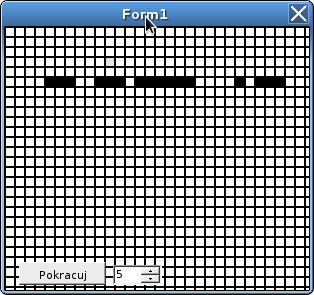
\includegraphics[width=0.7\textwidth]{./img/gol1}
 \label{gol1}
 \caption{The initial state of 'Life' (at t=0)}
\end{figure}

%The evolution of grid for our particular initial state is shown in figure blabla.\\  


\begin{figure}
 \centering
 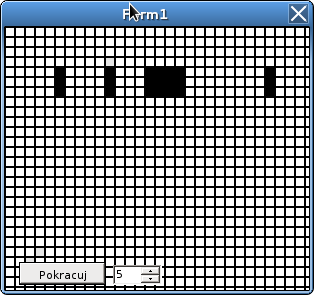
\includegraphics[width=0.7\textwidth]{./img/gol2}
 \label{gol2}
 \caption{t=1}
\end{figure}

\begin{figure}
 \centering
 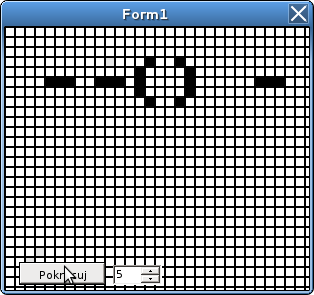
\includegraphics[width=0.7\textwidth]{./img/gol3}
 \label{gol2}
 \caption{t=2}
\end{figure}

Now we press 'Pokracuj' button and let the the Life evolve.
In the discrete time steps, the grid is changing.
We see that some cells are dying, but some cells are getting alive. 
What is the rule that kills the cell or leave it be? 

\begin{enumerate}
\item If the cell is alive, and 2 or 3 neighbouring cells are alive, the cell will stay alive in the next step. Otherwise it will die.
\item If the cell is dead, and \textbf{exactly} 3 neighboring cells are alive, the cell will get alive in the next step. Otherwise, it stays dead.

\end{enumerate}
We see that the rule involves only the state of the certain cell and the states of its eight neighboring cells.


Let us proceed from this simple example to more general setting.
In the next chapter, we will generalize main features of 'Life' and formally define the cellular automaton.
%In the next chapter, we will generalize main feature of 'Life'
%Let us generalize this example into formal definition of cellular automaton.

\section{Cellular automaton in general}

\begin{enumerate}
\item \textbf{Position of cells:}

Instead of 2D rectangular grid of 'Life',
cells might be arranged in arbitrary N dimensional
regular grid, not necessary rectangular. 
(Regularity follows from definition of Kubrid. In general, cells might be positioned really wildly,
e.g. on Penrose lattice, or arbritrary as proposed by Richard P. Feynman).

\item \textbf{Set of cell states Q:}

In 'Life' cells can be dead or alive (set of states has cardinality 2). 
In general CA, set of states can be any finite set Q of cardinality K.
%cell can be in one of K states from the finiteset of states. 
%We will mark set of states Q, and use this in definition of upgrade rule later.
\bigskip

\item \textbf{Neighborhood:}

In 'Life', state of the cell in the next step was determined
by 8 neighbouring cells. We call these cells neighborhood of range r = 1 (in the distance of 1 cell).
For general CA, we might consider neighborhood
with arbitrary range.
(Neighborhood with r = 2 in 'Life' would involve 9+16=25 cells).

\item \textbf{Update rule:}

Update rule is an arbitrary bounded mapping U from Neighborhood to the set of states Q.
Since the state of the Cell is determined only by the state of its Neighborhood, update rules in CA are local.

\end{enumerate}


\section{The most basic cellular automaton} 

In middle 1980s on the prestigious Princeton institute,
Stephen Wolfram and his assistants were performing unusual computer experiments. They were simulating the evolution of the $1D$ cellular automata and they were analyzing the patterns they obtained \cite{levy} (to a despair of their senior colleagues, who did not understand this "new kind of science")\cite{wolfram}.

The most basic, one dimension cellular automaton we can imagine, is the two state automaton with range $r=1$.

One dimensional indicates that the cells are arranged in the row, see Figure \ref{1d}

\begin{figure}[htbp]
 \centering 
 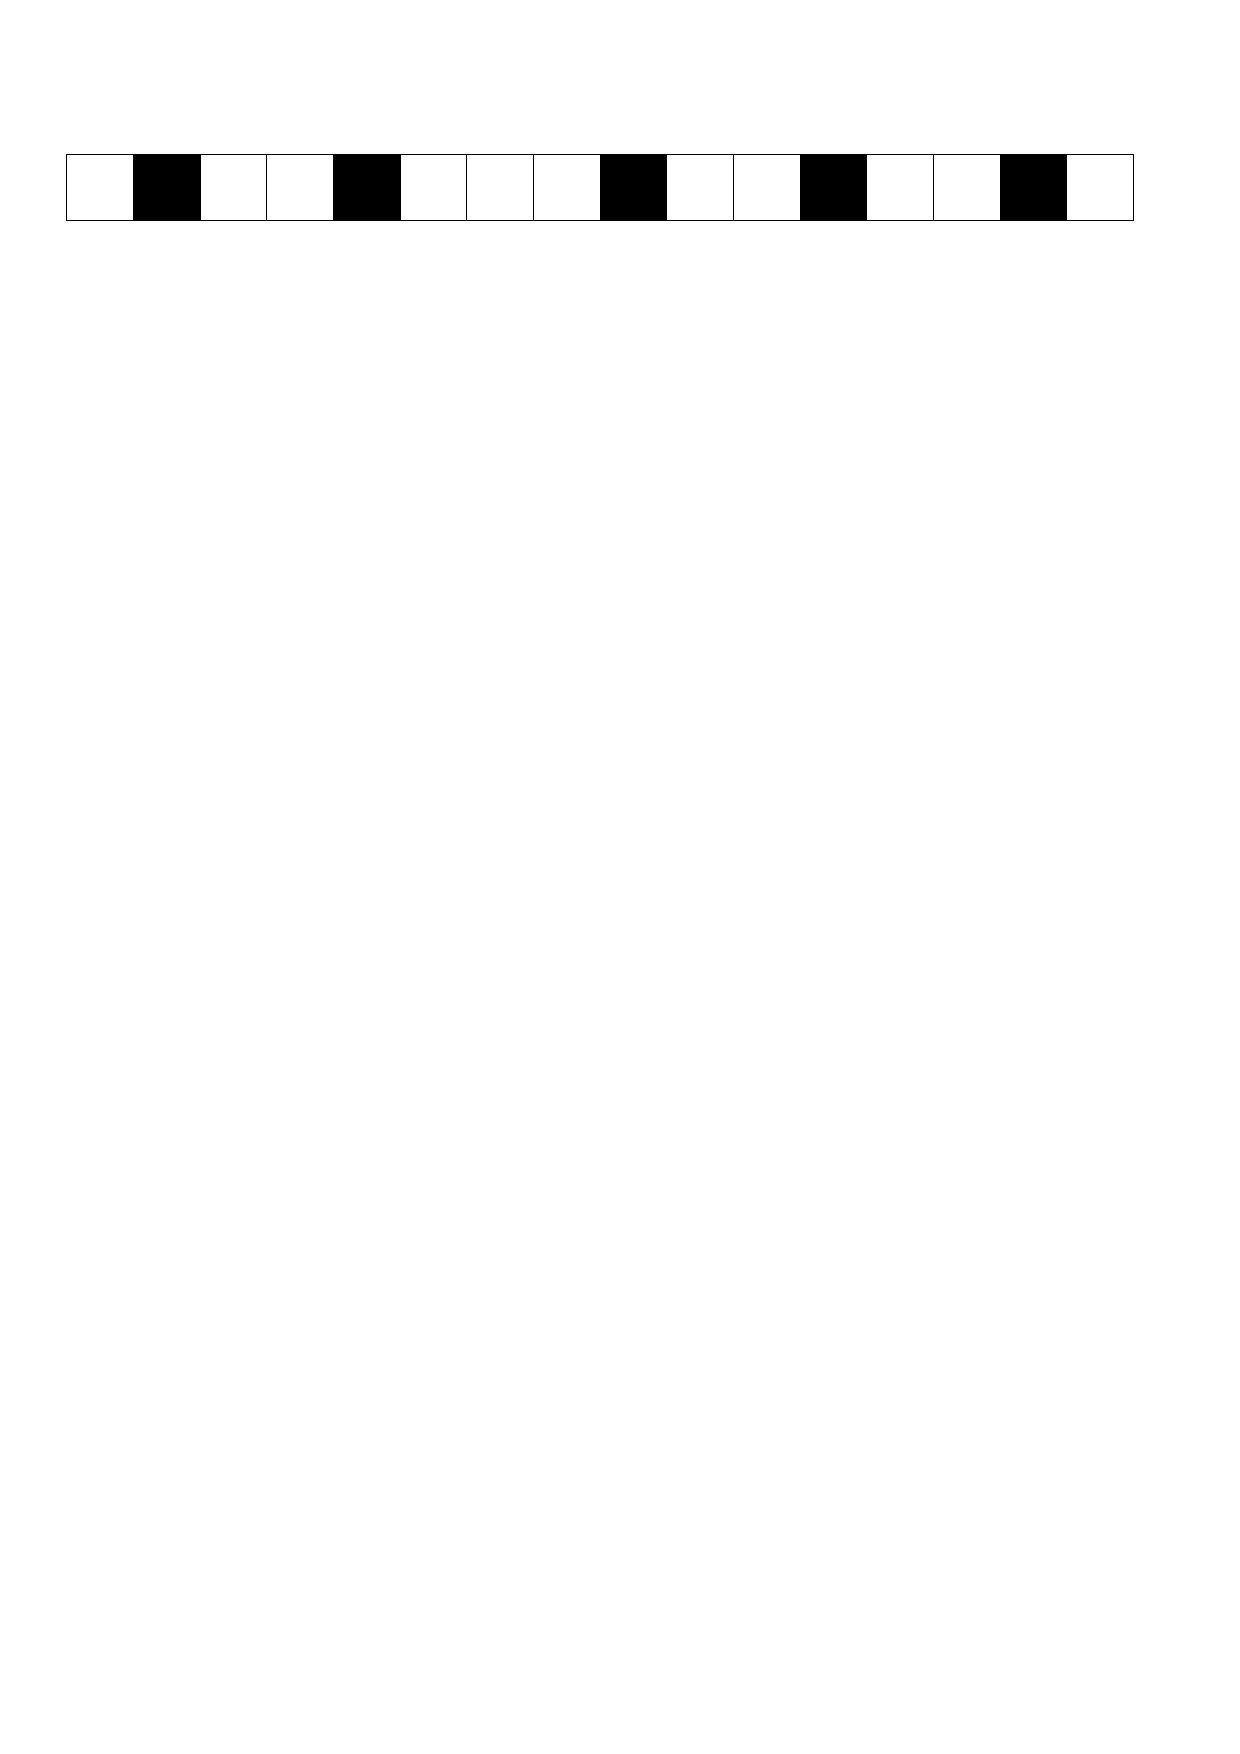
\includegraphics[width=0.9\textwidth]{./img/1Dline}
 \label{1d}
 \caption{A time-step of one dimensional cellular automaton}
\end{figure}

Range r=1 means that in update rule, we consider only the closest neighbors of the cell (one cell to the left, and one cell to the right).

Example of an update rule is shown the Table~\ref{rule90}.\\

\begin{table}[htbp]
 \centering
 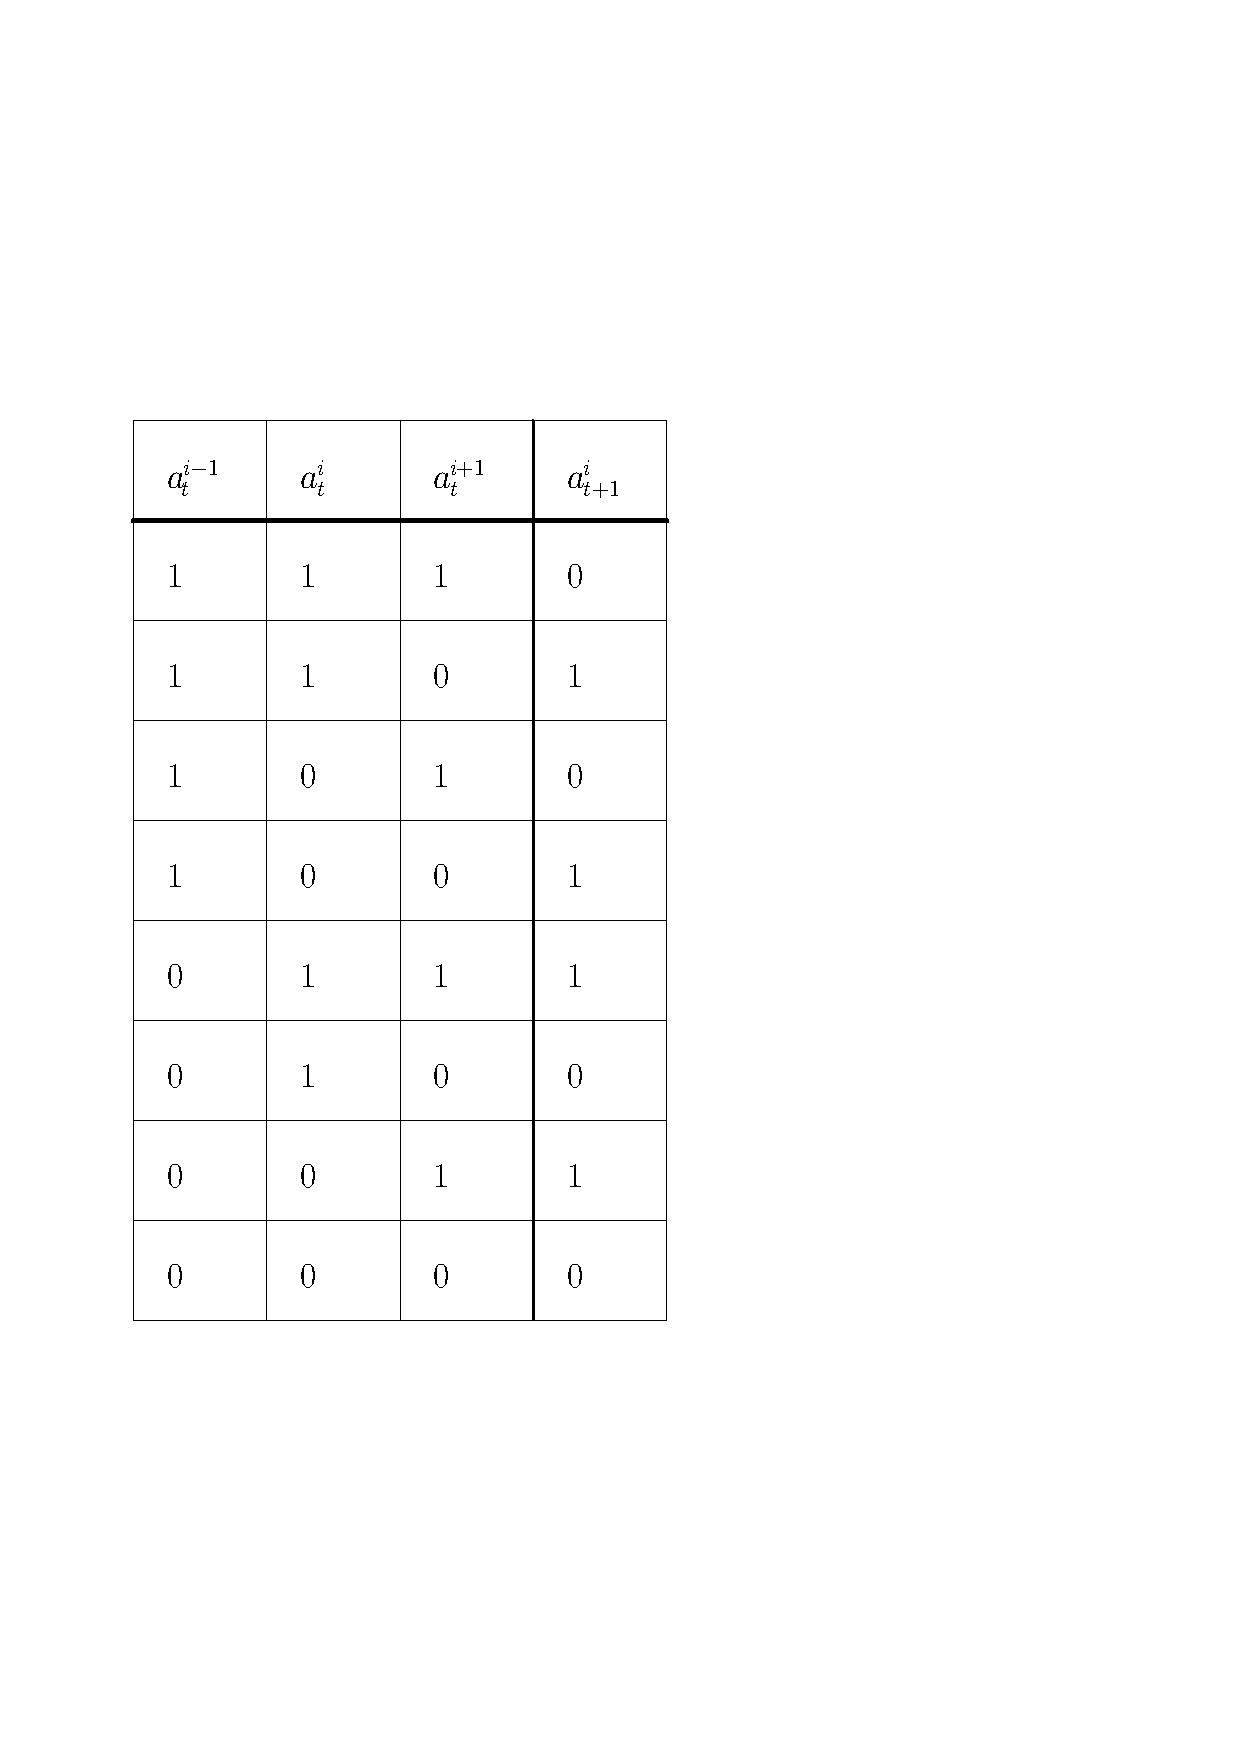
\includegraphics[width=0.4\textwidth]{./img/1Drule}
 \caption{Rule 90}
 \label{rule90}
\end{table}

%How many different update rules ("how many different Tables~\ref{rule90}")
%exist for this type of CA?

The three columns represent the state of a cell ($a_t^i$) and its left and right neighbor ($a_t^{i-1}$ and $a_t^{i+1}$ respectively). A living cell is denoted by 1, a dead cell is denoted by 0. The last column denotes the state of the middle cell ($a_i$) in the next step $t+1$. The sequence of $one$s and $zero$s in the last column is the binary $zapis$ of a number. In this particular case, the number is 90, hence the table specifies the Rule 90.
Since there is $2^8=256$ combinations for the last columns, there is $256$ rules for this most basic cellular automaton.
%For an automaton with $n$ states and range $r$, the rule involves $2r + 1$ cells, 

Let us take a look at some pictures of these cellular automata (the implementation of this automaton is simple, and these pictures were plotted by our program).

These pictures represent the evolution of cellular automata with rules 90, 30, 45 and 73.
The downer-most row is the initial configuration of CA, 
the 2nd row is configuration after 1st update etc.

\begin{figure}[!t]
 \centering
 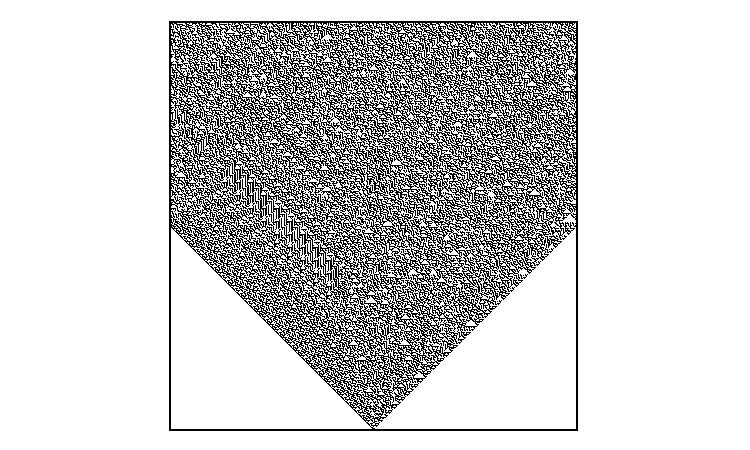
\includegraphics[trim = 40mm 0mm 0mm 0mm, width=1.7\textwidth]{./img/30_500}
 \caption{Rule 30}
\end{figure}

\begin{figure}[!b]
 \centering
 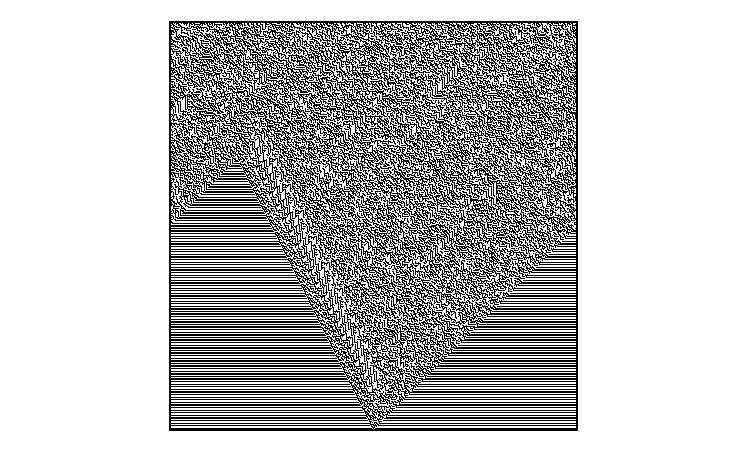
\includegraphics[trim = 40mm 0mm 0mm 0mm, width=1.7\textwidth]{./img/45_500}
 \caption{Rule 45}
\end{figure}

\begin{figure}
 \centering
 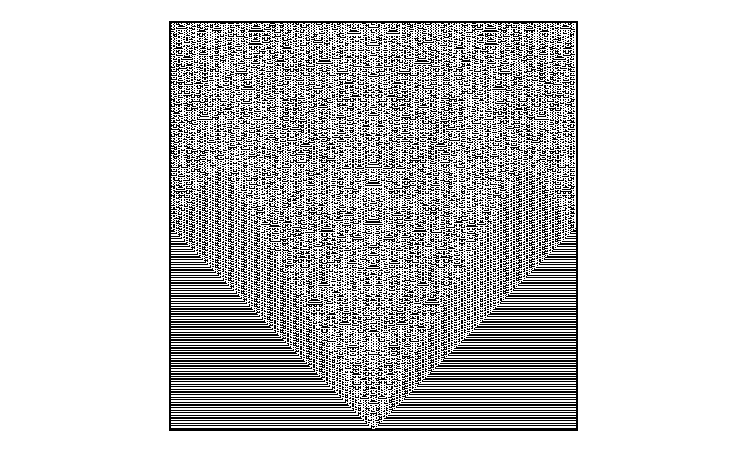
\includegraphics[trim = 40mm 0mm 0mm 0mm, width=1.7\textwidth]{./img/73_500}
 \caption{Rule 73}
\end{figure}


\begin{figure}
 \centering
 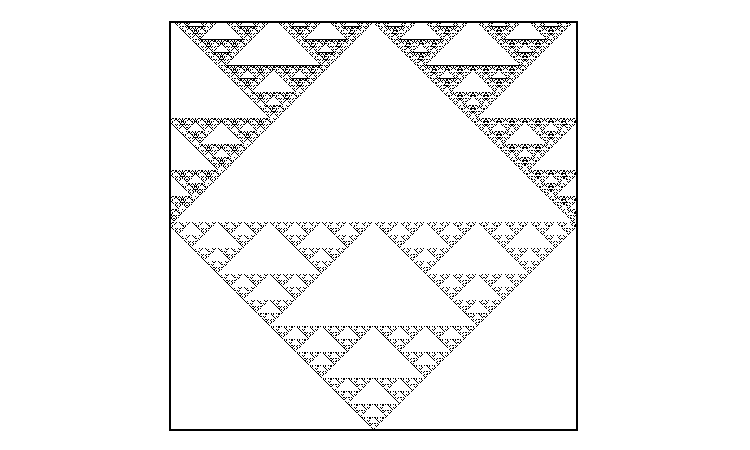
\includegraphics[trim = 40mm 0mm 0mm 0mm, width=1.7\textwidth]{./img/90_500}
 \caption{Sierpinski carpet - rule 90}
 \label{koberec}
\end{figure}


\begin{figure}
 \centering
 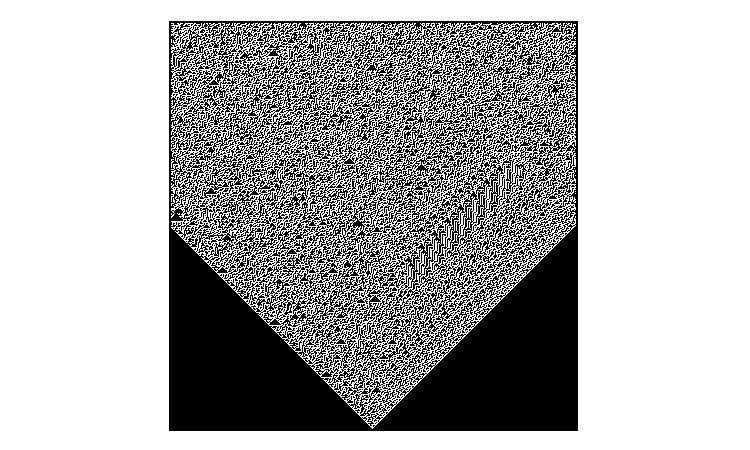
\includegraphics[trim = 40mm 0mm 0mm 0mm, width=1.7\textwidth]{./img/149_500}
 \caption{Sierpinski carpet - rule 149}
 \label{koberec}
\end{figure}

\begin{figure}
 \centering
 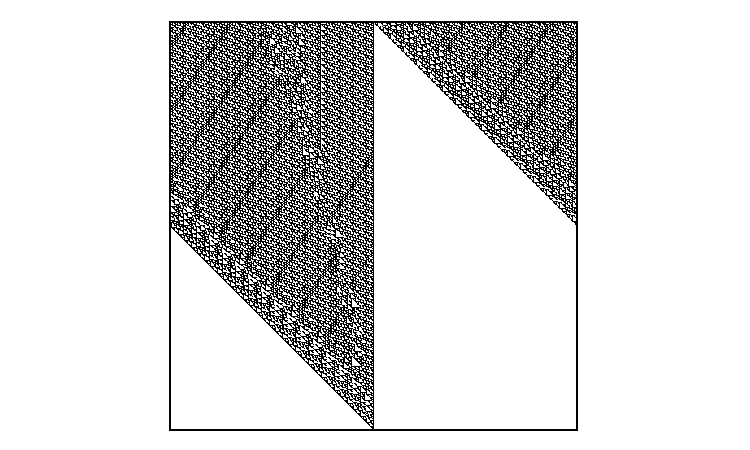
\includegraphics[trim = 40mm 0mm 0mm 0mm, width=1.7\textwidth]{./img/110_500}
 \caption{Rule 110}
\end{figure}

\begin{figure}
 \centering
 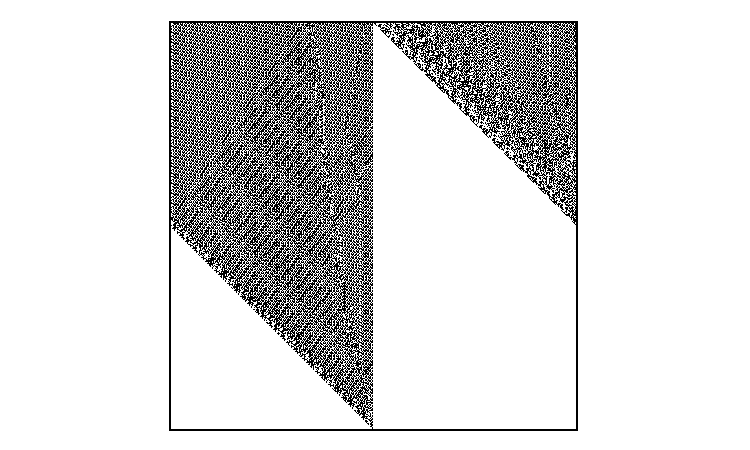
\includegraphics[trim = 40mm 0mm 0mm 0mm, width=1.7\textwidth]{./img/110_2000}
 \caption{Rule 110 -- $2000 \cross 2000$}
\end{figure}



First picture~\ref{koberec} is famous fractal known as Sierpinski carpet. Wolfram classified these 1D automata into four classes, based on the regularity of the pattern obtained.

Wolfram argues that variety of behavior seen even in these most simple CA rises suspitions, and encourage hope, that in the infinitely large world of possible CAs, there is CA that model any complex phenomena you can imagine.

In his visionary book New kind of Science, Wolfram even proposes Cellular automaton that would constitute a unified theory of the fundamental physics.
Although his ideas met with rejection among theorists (see \cite{aaronson}),
many other notable physicists are attempting to construct such cellular automaton \cite{hooft}).

Some of the basic construction principles for such automata are relevant also for our models, but mostly, we would diverge too far by further exploration.
Focus of our work is much more modest that CAs describing universe.
Our focus is on CAs that model flows of the fluids.

The connection of the cellular automata with flow of fluids is not obvious or formal.
It is found on the very general level.
What connects Navier-Stokes equations and CAs are their common symettries and conservation laws implied by these symetries.
In these symmetries lies not only beauty of this method, but their strongest advantage over other well-established CFD methods.